\documentclass[9pt]{beamer}

\usepackage[utf8]{inputenc}
\usepackage[T1]{fontenc}
\usepackage{lmodern}
\usepackage[french]{babel}

% Use the default theme and modify the color

\usepackage{amsmath}
\usepackage{xcolor}


\usecolortheme{seahorse}

% Define custom colors
\definecolor{myorange}{RGB}{255, 140, 0}
\definecolor{mywhite}{RGB}{0, 0, 0}

% Set general structure color to orange
\setbeamercolor{structure}{fg=myorange}

% Set frame title background color to orange
\setbeamercolor{frametitle}{bg=myorange, fg=mywhite}

% Customize title page colors
\setbeamercolor{title}{fg=mywhite}
\setbeamercolor{title graphic}{fg=mywhite}
\setbeamercolor{title separator}{fg=mywhite}
\setbeamercolor{subtitle}{fg=mywhite}

\title{Transport optimal, processus ponctuel déterminantaux et le noyau de Bergman}
\date{RECH202}
\author{William Driot}

\usepackage{graphicx}

\begin{document}

% Title page
\begin{frame}

\titlepage

\end{frame}\begin{frame}\frametitle{Processus ponctuels}

    \begin{center}

    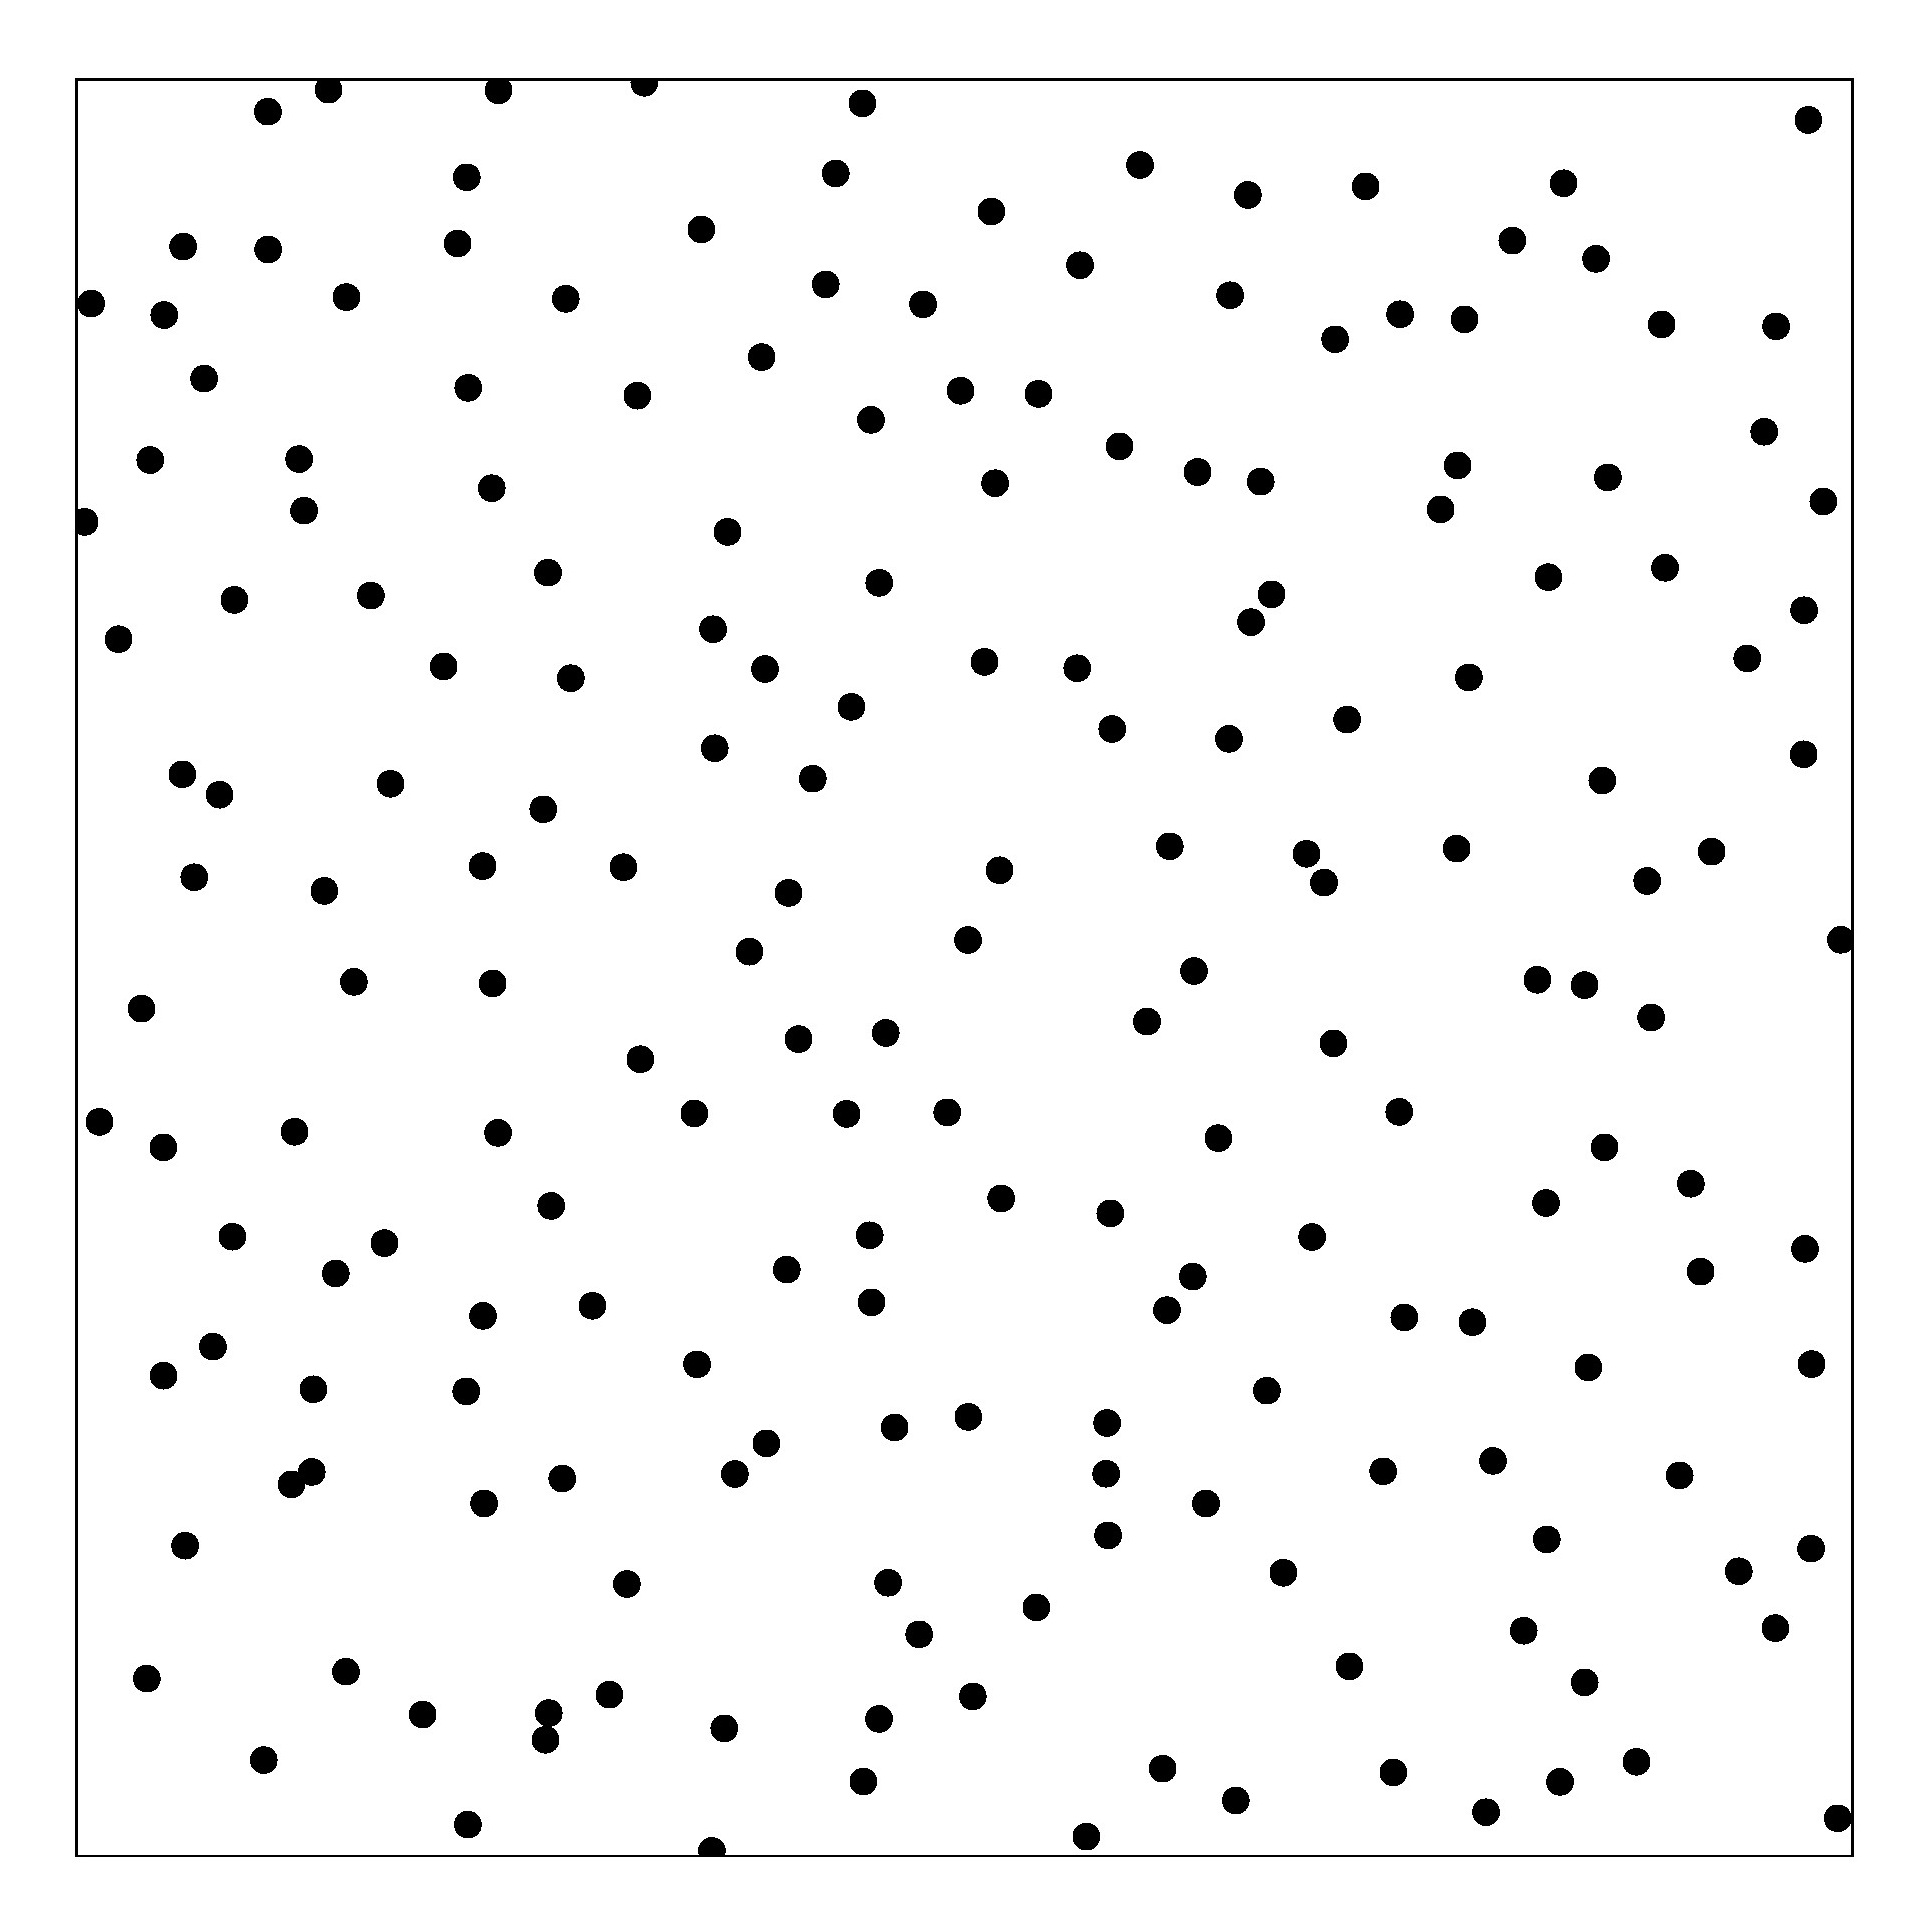
\includegraphics[scale=1]{Points trimmed.jpg}

    
    Un processus ponctuel est une variable aléatoire à valeur dans l'espaces des \og configurations \fg (= parties localement finies, de $ \mathbf C $ par exemple muni de la tribu engendrée par le topologie de la convergence vague).
    \end{center}

\end{frame}\begin{frame}\frametitle{Processus ponctuels déterminantaux}

    \textbf{Définition :}

    Un processus ponctuel sur $E$ est \textbf{déterminantal} de noyau $k : E^2 \to \mathbf C$ si ses fonctions de corrélation s'écrivent :
    \[
        \rho_n(x_1,...,x_n) = \mathrm{det}(k(x_i,x_j))_{1 \leqslant i,j \leqslant n}
    \]
    où $ k : E^2 \to \mathbf C $ est une fonction $L^2$.

\end{frame}\begin{frame}\frametitle{Théorème fondamental}

    \textbf{Théorème :} (fondamental)

    Considérons un DPP de noyau $k$, dont les valeurs propres sont dans $[0,1]$.

    D'après le théorème de Mercer, on peut écrire 
    \[ 
        k(x,y) = \sum_{i \in \mathbf N} \lambda_i \phi_i (x) \overline{\phi_i(y)}
    \] 
    où les $ (\lambda_i)_{i \in I} $ sont les valeurs propres de $K$ dans $[0,1]$.

    \bigskip

    La loi induite par $k$ est la même que celle induite en tirant $ (B_i)_{i \in I} $ des variables aléatoires de Bernoulli indépendantes de paramètres respectifs $ \lambda_i $, puis la loi induite par 
    \[
         k_B(x,y) = \sum_{j \in I} B_j \phi_j(x) \overline{\phi_j(y)}
    \]

\end{frame}\begin{frame}\frametitle{Noyaux de Ginibre et Bergman}

    \bigskip

    Noyau de Ginibre sur $ E = \mathbf C $ : 
    
    $$ k(x,y) = \frac 1 \pi e^{x \overline y} e^{- \frac 1 2 (|x^2| + |y|^2)} = \sum_{n \in \mathbf N} \phi_n(x) \overline{\phi_n(y)}$$

    $$ \phi_n(x) = \frac{1}{\sqrt{\pi n!}} e^{- \frac 1 2 |z|^2} z^n $$

    \bigskip

    Noyau de Bergman sur $ E = \mathcal B(0,1) \subset \mathbf C $ :

    $$ k(x,y) = \frac{1}{\pi(1-x\overline y)^2} = \frac 1 \pi \sum_{k=0}^\infty (k+1)(x \overline y)^k $$

\end{frame}\begin{frame}\frametitle{Noyaux de Ginibre et Bergman}

    \begin{center}

    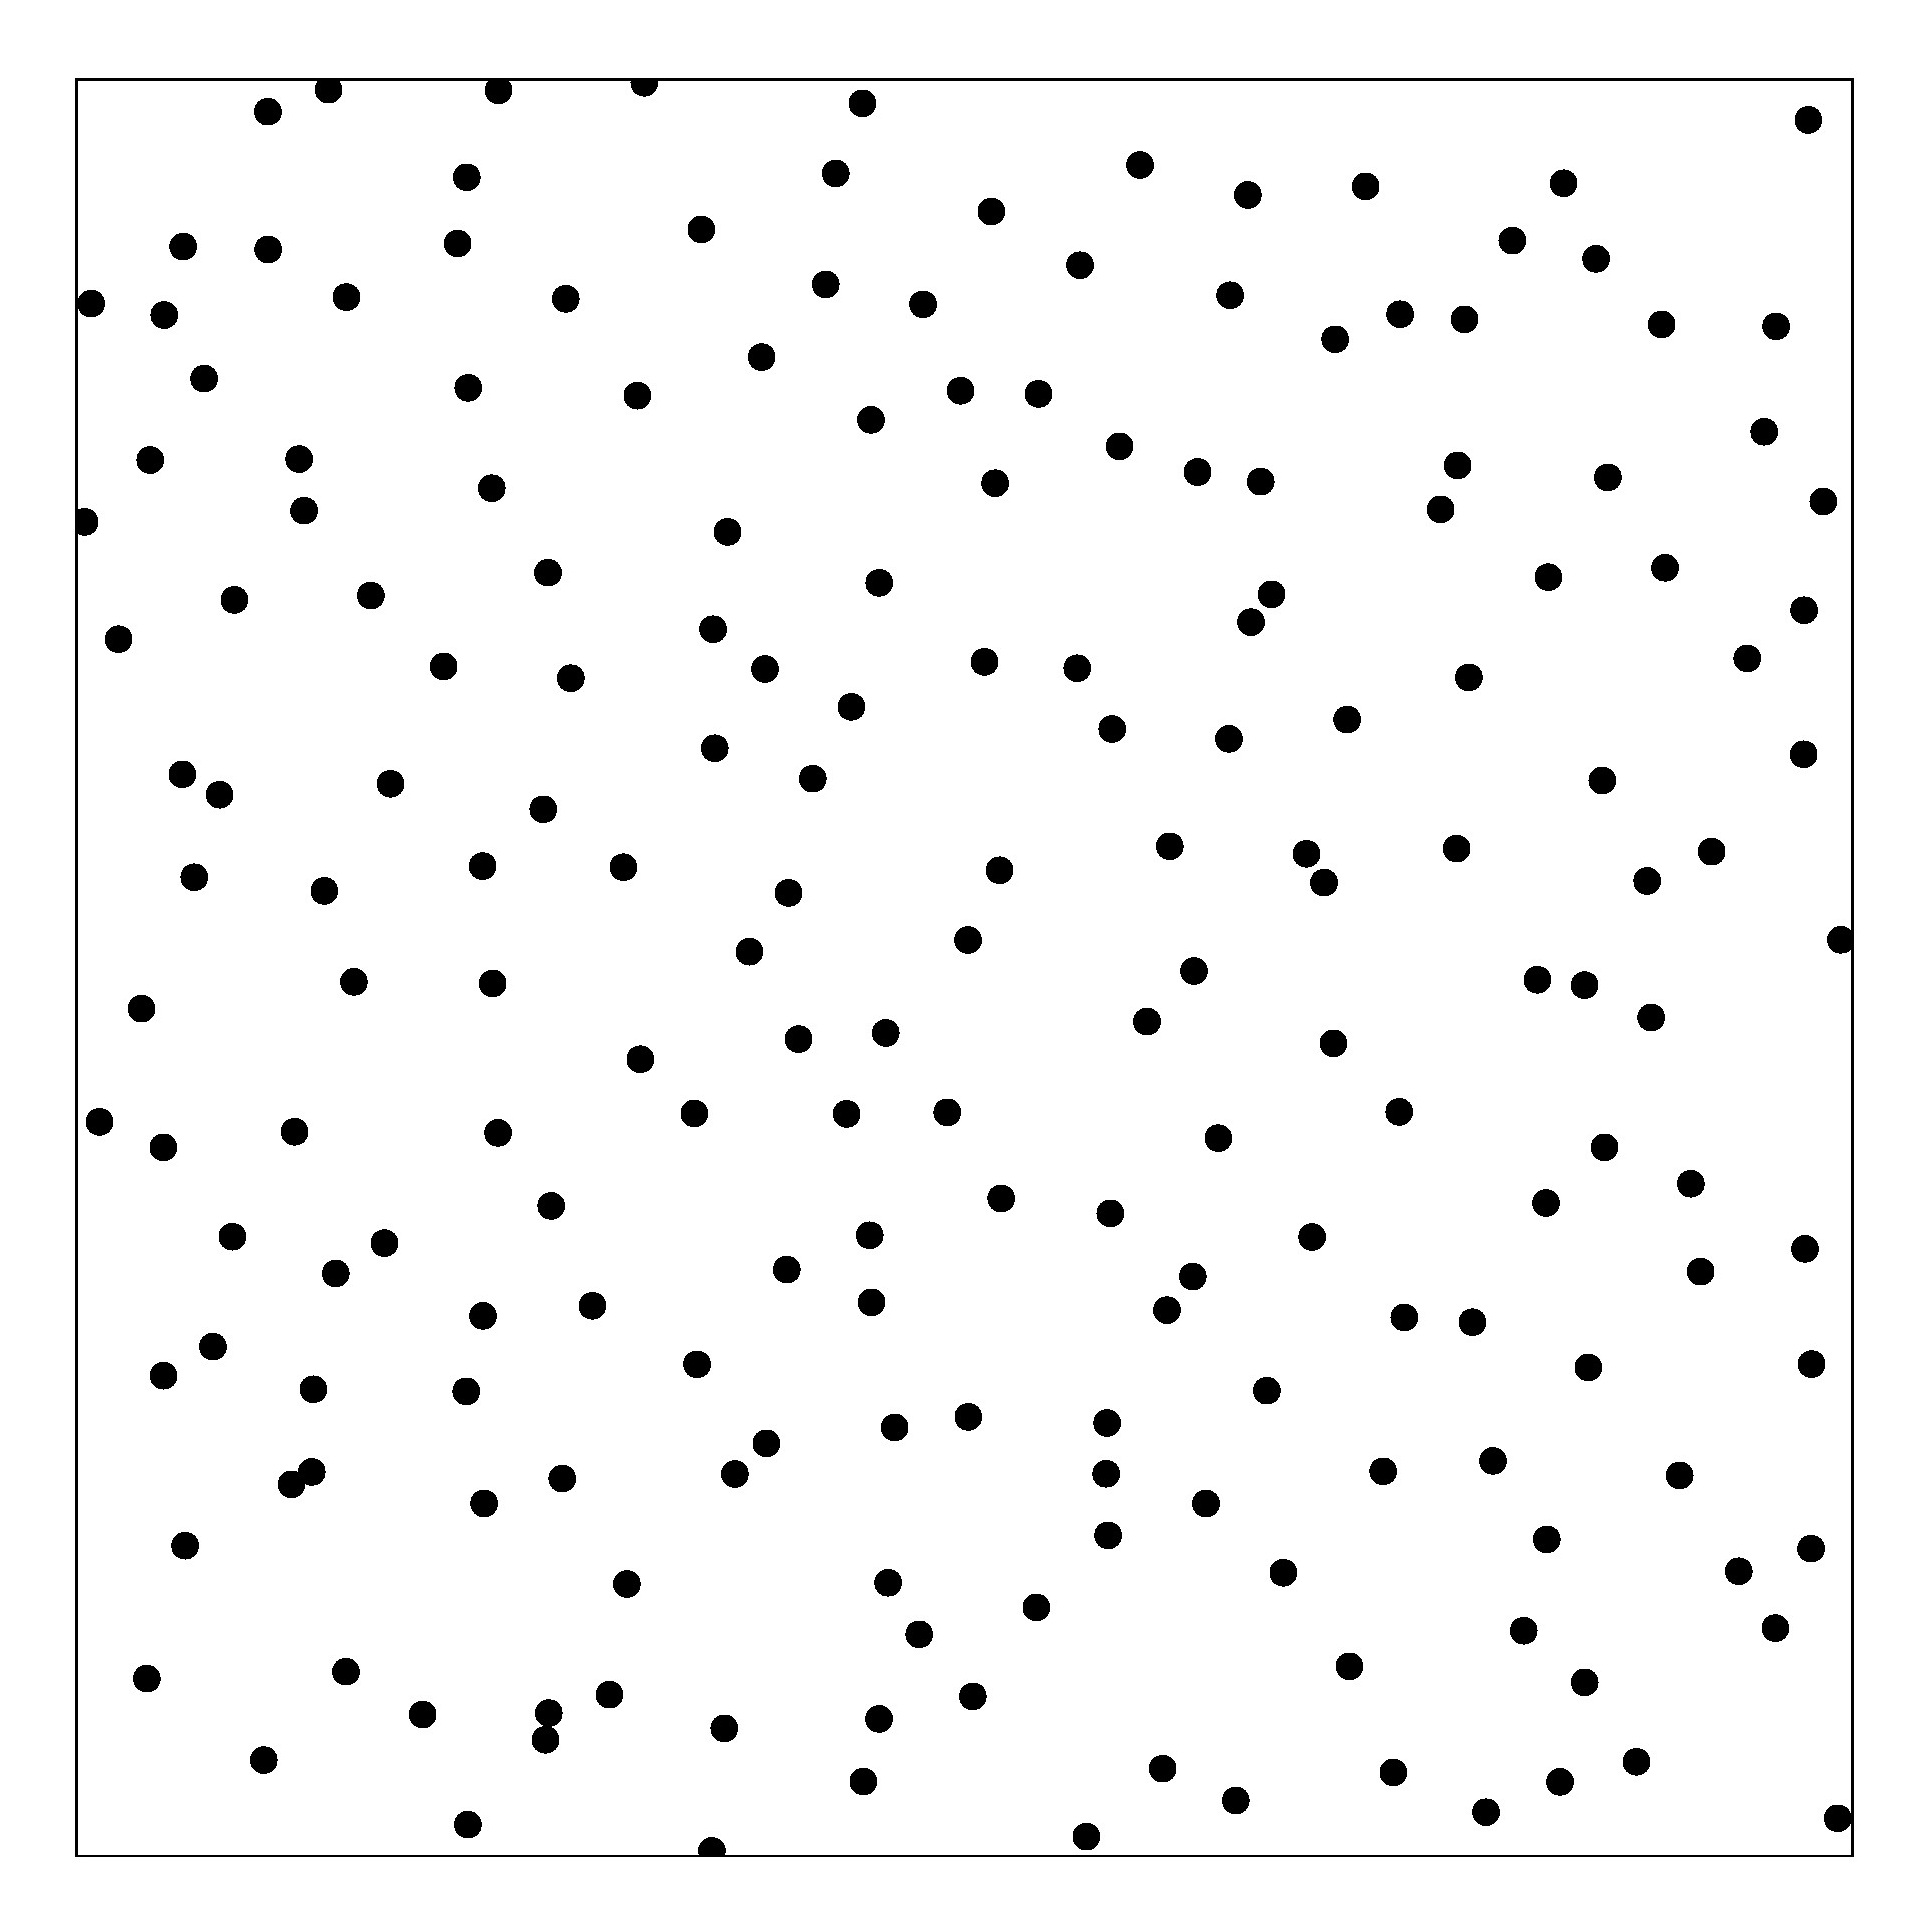
\includegraphics[scale=0.7]{Points trimmed.jpg} 

    Ginibre

    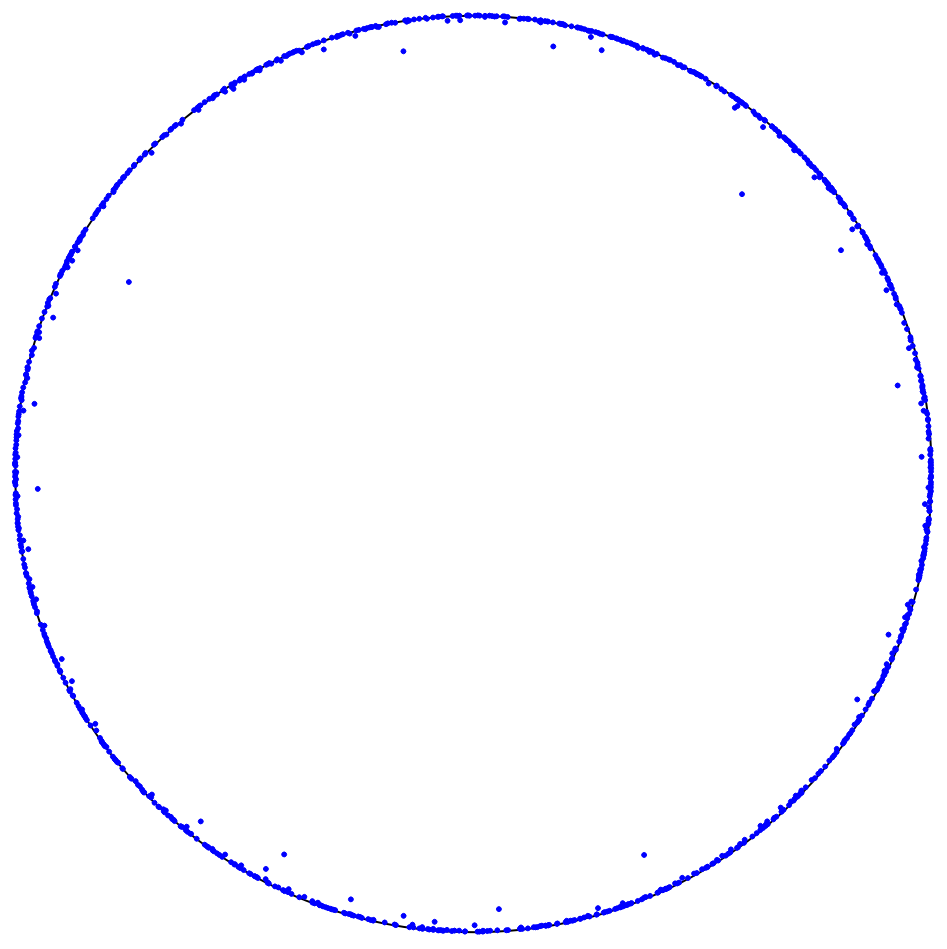
\includegraphics[scale=0.15]{bergman.png} 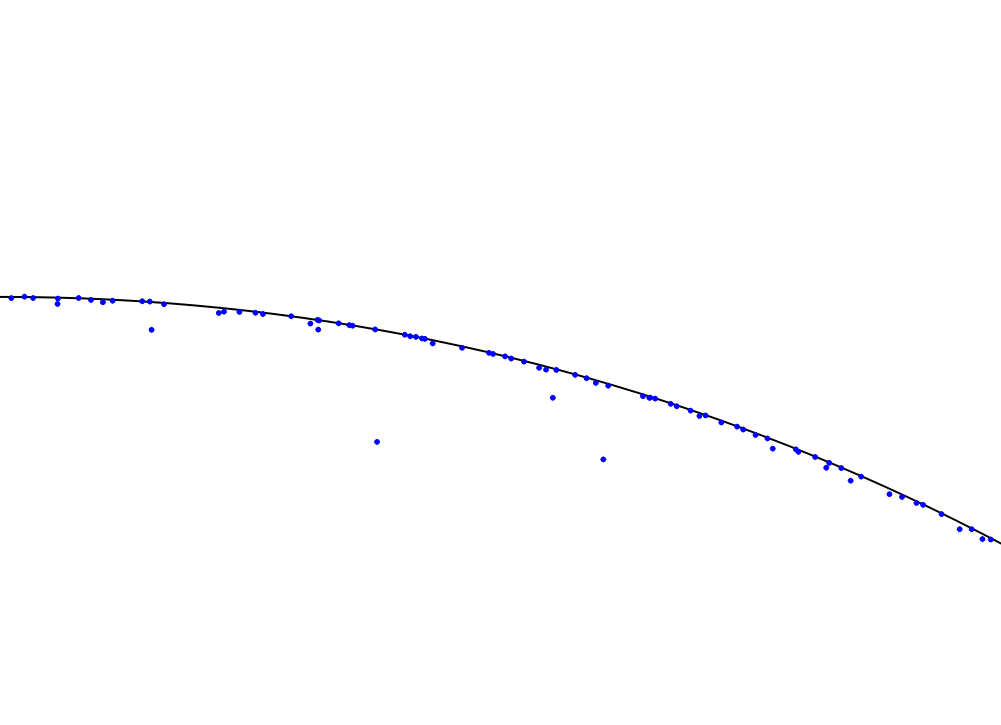
\includegraphics[scale=0.15]{bergman_zoom.png} 

    Bergman

    \end{center}

\end{frame}\begin{frame}\frametitle{Simulation}

    \textbf{Problème :} DPPs stationnaires (Ginibre) : les points s'étendent sur $ \mathbf C $ tout entier. 

    \medskip 

    \textbf{Solution :} Restriction à une partie $ \Lambda $, opération mathématique qui construit une variante du DPP pour laquelle il n'y a que des points dans $ \Lambda $.

    \medskip

    \textbf{Problème :} ces DPPs présentent une infinité de points presque sûrement. 

    \medskip

    \textbf{Solution :} Troncation : On considère l'écriture de Mercer $ \sum_{k=0}^{N-1} $ au lieu de $ \sum_{n=0}^\infty $

    \textbf{Question :} Ils sont donc impossibles à simuler stricto-censu. Mais on simule des processus différents ! Ce ne sont plus les mêmes lois !

    \begin{center} $ \rightarrow $ \textbf{Quelle sont les pertes induites par de telles modifications ?}  \end{center}

\end{frame}\begin{frame}\frametitle{1er résultat : Noyau de Bergman restreint}

    \textbf{Théorème.} Soit $\mathcal{B}(0, R)$ le disque de $ \mathbf C $ de centre $0$ et de rayon $R$. On peut (et c'est assez rare pour le souligner) calculer explicitement les valeurs propres et les fonctions propres, et donc la décomposition de Mercer du noyau $k^R(x,y)$ du DPP de Bergman retreint à $\mathcal{B}(0, R)$ :
    \[
    k^R(x,y) = \sum_{n \ge 0} \lambda_n^R \phi_n^R(x) \overline{\phi_n^R(y)},
    \]
    où les valeurs propres sont les 
    \[
    \lambda_k^R = R^{2k+2},
    \]
    et les fonctions propres
    \[
    \phi_k^R : x \mapsto \sqrt{\frac{k+1}{\pi}} \frac{1}{R^{k+1}} x^k.
    \]

    Cet opérateur restreint est à trace donc il présente un nombre \textit{fini} de points p.s. ! 

\end{frame}\begin{frame}\frametitle{Troncation du Bergman projeté}

    \textbf{Rappel :} On ne peut pas simuler un nombre infini de variables aléatoires de Bernoulli. Où s'arrêter alors ?

    \medskip 

    \textbf{Théorème :} Soit
    \[
    N_R := \sum_{n=0}^\infty R^{2n+2} = \frac{R^2}{(1-R)(1+R)}.
    \]
    Soit $\mathfrak{S}^R$ la loi de Bergman restreint au disque compact de rayon $R$ centré en $0$, et $\mathfrak{S}_\alpha^R$ la loi de sa troncation à $\alpha$ points. Si on tronque à $\beta N_R$ points, on a
    \[
        \mathcal{W}_{KR}(\mathfrak{S}^R, \mathfrak{S}_{\beta N_R}^R) \leqslant N_R e^{-2\beta g(R)}
    \]
    où $ g(R) = \frac{R^2}{1+R} $ 

    \textbf{Notations :} $ \mathfrak{S}^R $ = Bergman restreint à $ \mathcal B(0,R) $, $ \mathfrak{S}_{N}^R $ = Bergman restreint tronqué à $N$ points

\end{frame}\begin{frame}\frametitle{Distance de Kantorovitch-Rubinstein $ \mathcal W_{KR} $}

    \textbf{Distance de Kantorovitch-Rubinstein : } Pour $ E =$ espace des configurations muni de la distance de variation totale $ d(\xi, \zeta) = | \xi \Delta \zeta| $;
    \[
    \mathcal{W}_{KR}(\mu, \nu) = \inf_{\substack{\text{law}(\xi)=\mu \\ \text{law}(\zeta)=\nu}} \mathbf{E}(|\xi \Delta \zeta|) = \inf_{\substack{\text{law}(\xi)=\mu \\ \text{law}(\zeta)=\nu}} \mathbf{E}(d(\xi, \zeta)).
    \]

    C'est une distance entre lois de processus ponctuels issue du Transport Optimal.

\end{frame}\begin{frame}\frametitle{Troncation du Bergman projeté}

    \textbf{Théorème :} Soit
    \[
    N_R := \sum_{n=0}^\infty R^{2n+2} = \frac{R^2}{(1-R)(1+R)}.
    \]
    Soit $\mathfrak{S}^R$ la loi de Bergman restreinte du disque compact de rayon $R$ centré en $0$, et $\mathfrak{S}_\alpha^R$ la loi de sa troncation à $\alpha$ points. Si on tronque à $\beta N_R$ points, on a
    \[
        \mathcal{W}_{KR}(\mathfrak{S}^R, \mathfrak{S}_{\beta N_R}^R) \leqslant N_R e^{-2\beta g(R)}
    \]
    où $ g(R) = \frac{R^2}{1+R} $

    \textbf{Corollaire :}
    \[
    \mathbf{P}(\mathfrak{S}^R \neq \mathfrak{S}_{\beta N_R}^R) \leqslant N_R e^{-2\beta \frac{R^2}{1+R}}.
    \]

    Autrement dit, tronquer au delà de $ N_R $ induit des distances (de Wasserstein) exponentiellement faibles entre les lois des processus. Donc $ N_R $ est un bon choix.

\end{frame}\begin{frame}\frametitle{Démarche : pourquoi ce $ N_R $ là ? }

    \textbf{Théorème :} (Decreusefond, Moroz, 2021)
    
    Soit $R > 0$. On tronque le Ginibre projeté à $ N_R = (R+c)^2 $ points. Soient $ \xi^R $ et $ \xi^R_{N_R} $ des DPPs ayant ces lois (projeté / projeté et tronqué). Alors
    \[
         \mathcal W_{KR}(\xi^R, \xi^R_{N_R}) \leqslant \sqrt{\frac{2}{\pi}} R e^{-c^2}
    \]

    \textbf{Observation :} En fait, il s'avère que $ R^2 $ n'est autre que l'espérance du nombre de points !

    \begin{center}

    $ \rightarrow $ ce résultat majore la \textbf{déviation} du nombre de points autour de son espérance. 

    Le nôtre aussi, et en est un analogue pour le processus de Bergman.

    \end{center}

\end{frame}\begin{frame}\frametitle{Convergence au sens de Wasserstein}

    \textbf{Question :} Notre borne ne tend pas vers $0$ quand $ R \to 1^-$. Mais a-t-on quand même convergence au sens de Wasserstein?
    \[ 
        \mathcal W_{KR} ( \mathfrak S^R, \mathfrak S^R_{N_R}) \xrightarrow[R \to 1^-]{} 0
    \]

    \textbf{Autre question :} Tronquer à l'espérance ? Mais, par définition, une v.a. peut dépasser son espérance, non ?

    \textbf{Proposition :} Pour tout $ \delta > 0 $, si on tronque à $ N_R^{1+\delta} $, on a 
    \[ 
        \mathcal W_{KR} ( \mathfrak S^R, \mathfrak S^R_{N_R^{1+\delta}}) \xrightarrow[R \to 1^-]{} 0
    \]

    \textbf{Proposition :} Plus généralement on a toujours la convergence au sens de Wasserstein si
    \[
        N_R \sim_{R \to 1^-} \frac{1}{(1-R)^{1+\delta}} 
    \]
    et encore plus généralement, la borne tend vers 0 si et seulement si
    \[ 
        2N_R  \log(R) - \log(1-R) \xrightarrow[\varepsilon \to 0^+]{} - \infty 
    \]
    \begin{center} 
        $ \rightarrow $ CNS sur la croissance en $R$ de $ N_R $ pour le choix du nombre de points (troncation) pour que la borne tende vers $0$ (CS de Wasserstein convergence) 
    \end{center}

\end{frame}\begin{frame}\frametitle{Convergences en loi}

    \textbf{Théorème.} On a 
    \[
    \mathfrak{S}_N^R \xrightarrow[N \to \infty]{} \mathfrak{S}^R,
    \]
    en loi.

    \bigskip
    
    En particulier, $ \mathfrak{S}_{N_R}^R \xrightarrow[N \to \infty]{} \mathfrak{S}^R $ dès que $ N_R \xrightarrow[R \to 1^-]{} \infty$, donc en particulier pour notre $ N_R$ précédent.

    \bigskip

    \textbf{Théorème.} On a, dès que $ N_R \xrightarrow[R \to 1^-]{} +\infty $ (erreur ici! dans la preuve aussi!)
    \[
        \mathfrak{S}_{N_R}^R \xrightarrow[R \to 1^-]{} \mathfrak{S},
    \]
    en loi. 

\end{frame}\begin{frame}\frametitle{Restriction à un anneau (cf. observations)}

    \textbf{Théorème.} Soit $T(r,R)$ l’anneau compact centré en 0, de rayon intérieur $r$ et de rayon extérieur $R$. La décomposition de Mercer du noyau $k_{r,R}(x,y)$ du processus ponctuel déterminantal de Bergman restreint à $T(r,R)$ est

    \[
        k_{r,R}(x,y) = \sum_{n \ge 0} \lambda_n^{r,R} \phi_n^{r,R}(x) \overline{\phi_n^{r,R}(y)}
    \]
    où les valeurs propres sont
    \[
    \lambda_k^R = R^{2k+2} - r^{2k+2}
    \]
    et les vecteurs propres
    \[
    \phi_k^R: x \mapsto \sqrt{\frac{k+1}{\pi(R^{2k+2} - r^{2k+1})}} x^k
    \]

    \bigskip

    Autrement dit, on peut restreindre à un anneau aussi. D'ailleurs, 

    \textbf{Proposition.} On peut calculer la loi de la plus petite distance entre un point et l'origine est $ \sim x^2$ quand $ x\to 0$.

    Ceci montre qu'il y a de toute manière très peu de points à l'origine.

\end{frame}\begin{frame}\frametitle{Restriction à un anneau de rayon extérieur 1 ?}

    \textbf{Notation :} Dans la suite, on note 
    \[
    Z(A) = \{z \in \mathbb{C}, |z| \in A\}.
    \]

    Ces parties sont invariantes par rotation.

    \textbf{Théorème :}
    
    La restriction du Bergman à toute région de la forme \( Z(A) \), \( A \subset [0,1] \) contenant \( Z([1-\varepsilon, 1]) \) présente presque sûrement un nombre infini de points.

    Autrement dit, pour la simulation, il faut abandonner l'idée de vouloir absolument simuler les points au voisinnage du cercle unité $ Z(\{1\}) $.

\end{frame}\begin{frame}\frametitle{Simuler les points au voisinnage du cercle unité ?}


    \textbf{Théorème.} Soit \( (u_n)_{n \geqslant 0} \) une suite de nombres positifs telle que  
\[ 
    \sum_{n \ge 0} u_n < +\infty. 
\]  
Soient \( (a_n)_{n \in \mathbf{N}} \) et \( (b_n)_{n \in \mathbf{N}} \) deux suites à valeurs dans \( (0,1) \) avec \( 0 < a_0 < b_0 < 1 \) qui satisfont la relation de récurrence suivante :  
\[
\forall n \in \mathbf{N}, 
\left\{
\begin{aligned}
    a_{n+1} &\in (b_n, 1) \\[6pt]
    b_{n+1} &= \sqrt{ \frac{a_{n+1}^2 + u_n (1 - a_{n+1}^2)}{a_{n+1}^2 + (1 + u_n)(1 - a_{n+1}^2)} }
\end{aligned}
\right.
\]
Alors le processus ponctuel déterminantal de Bergman restreint à  
\[
    Z\left( \bigcup_{n \ge 0} [a_n, b_n] \right)
\]
présente presque sûrement un nombre fini de points. De plus, si on choisit $ a_n \to 1 $, cette région adhère au cercle unité, et si on prend $ b_0 \geqslant 1 - \delta < 1 $, la mesure de Lebesque de cette région est proche de $ \pi $ !

\end{frame}\begin{frame}\frametitle{Résultats généraux autour des DPPs}

    \textbf{Théorème.} Soit $ \mathfrak S$ un DPP et $ \mathfrak S_n $ sa troncation à $n$ points. On note $ m_n $ la moyenne du nombre de points de $ \mathfrak S_n $ et $ \sigma^2_n $ sa variance. 

    Alors 
    \[
        \frac{| \mathfrak S_n | - m_n }{\sigma_n^2\sqrt n} \xrightarrow[n \to \infty]{} \mathcal N (0,1)
    \]
    en loi.

\end{frame}\begin{frame}\frametitle{Résultats généraux autour des DPPs}

    \textbf{Théorème.} Soit \(\mathfrak{S}\) un processus ponctuel déterminantal. Supposons que l'opérateur intégral associé soit à trace. Notons \(m\) le nombre moyen de points de \(\mathfrak{S}\). 
    
    Alors, \(m\) est fini, et pour tout \(c \in (0,1)\), on a  
    \[
        \mathbf{P}(|\mathfrak{S}| \leqslant (1-c)m) \leqslant \exp\big(-m \big(c + (1-c) \log(1-c)\big)\big),
    \]
    et pour tout \(c > 0\),  
    \[
        \mathbf{P}(|\mathfrak{S}| \geqslant (1+c)m) \leqslant \exp\big(-m \big((1+c) \log(1+c) - c\big)\big).
    \]

\end{frame}\begin{frame}\frametitle{Fonctions de corrélation}

    \textbf{Définition :}

    Soit $\xi $ un processus ponctuel, $ \lambda $ une mesure de référence sur $E$. $ \xi $  admet $(\rho_n) $ pour fonctions de corrélations si pour toutes parties $A_1,...,A_n$ mesurables \textit{deux à deux disjointes} de $E$, on a $$ \mathbb E \left[ \prod_{k=1}^n \xi(A_k) \right] = \int_{A_1\times ... \times A_n} \rho_n(x_1,...,x_n) \mathrm d \lambda^{\otimes n} $$ Les fonctions de corrélation $ (\rho_n)_{n \in \mathbf N}$ caractérisent la loi d'un processus ponctuel.

\end{frame}\begin{frame}\frametitle{Écriture de Mercer}

    \textbf{Théorème :} (Mercer)

    \bigskip

    Sur $ (E, \mu) $, soit $ k \in L^2 $ un noyau. On suppose que $k$ est de type positif et que l'opérateur intégral $K$ associé à $k$ est auto-adjoint.

    \bigskip

    Alors les valeurs propres $ \lambda_i $ de l'opérateur intégral $K$ associé à $k$ sont positives, et il existe une base hilbertienne $(\phi_n)_{n\in\mathbf N}$ de $L^2$ formée de vecteurs propres pour $K$, telle que 
    \[
        k(x,y) = \sum_{n \in \mathbf N} \lambda_n \phi_n(x) \overline{\phi_n(y)} 
    \]

\end{frame}\end{document}